\documentclass[12pt]{article}

\usepackage{apuntes-estilo}
\usepackage{fancyhdr,lastpage}
\usepackage{color,colortbl}
\usepackage{verbatim}

\def\maketitle{

% Titulo 
 \makeatletter
 {\color{bl} \centering \huge \sc \textbf{
 El primer programa embebido\\ 
\large \vspace*{-8pt} \color{black} Programación de Sistemas Embebidos
 \vspace*{8pt} }\par}
 \makeatother


% Autor
 \makeatletter
 {\centering \small 
 	Departamento de Ingeniería de Computadoras \\
 	Facultad de Informática - Universidad Nacional del Comahue \\
 	\vspace{20pt} }
 \makeatother

}

% Custom headers and footers
\fancyhf{} % clear all header and footer fields
\fancypagestyle{plain}{\fancyhf{}}
  	\pagestyle{fancy}
 	\lhead{\footnotesize El primer programa embebido - Departamento de Ingeniería de Computadoras}
 	\rhead{\footnotesize \thepage\ }	% ''Page 1 of 2''

\def\ti#1#2{\texttt{#1} & #2 \\ }



\begin{document}

\thispagestyle{empty}
\maketitle
\setlength{\parindent}{0pt}



En este capítulo realizaremos programación embebida directa a través de un ejemplo.
Nuestro ejemplo es similar, en espíritu, al programa 'Hello, World!' que puede encontrar al comienzo de la mayoría de los libros de programación
Tambien, explicaremos las razones por la cual seleccionamos el programa particular
presentado en este capítulo, y especificamos las secciones de código que son dependientes del hardware.
El capítulo unicamente contiene el código fuente del programa. Se explica como compilar y ejecutar el programa en el capítulo siguiente.

\section *{Hello, World!}

Pareciera que todo libro sobre programación comienza con el mismo ejemplo -un programa que imprime 'Hello, World!' en la pantalla del usuario. Un ejemplo como este tan utilizado podría parecer aburrido.
Entre otras cosas, el ejemplo ayuda al lector a verificar la facilidad o dificultad con la que se pueden escribir programas sencillos en el ambiente de programación utilizado. En ese sentido, el programa 'Hello, World!' es muy útil como benchmark para los usuarios de lenguajes de programación y plataformas de computación.

Basados en el benchmark 'Hello, World!' los sistemas embebidos son las plataformas de computación mas desafiantes con las cuales trabajar. Incluso, en algunos sistemas embebidos podría ser imposible implementar el programa 'Hello, World!'. Y en los sistemas capaces de ejecutar un programa del estilo, el hecho de imprimir mensajes de texto usualmente es más un punto de llegada que el comienzo del aprendizaje.


Una presunción principal del ejemplo 'Hello, World!' es que existe algun tipo de dispositivo de salida en el cual las cadenas de caracteres puedan ser mostradas. Una ventana de texto en el monitor del usuario usualmente sirve para ese propósito. Pero, la mayoría de los sistemas embebidos no contienen un monitor o dispositivo de salida similar. Y para los que tengan , tipicamente, requieren una pieza especial de software embebido, llamado controlador de pantalla (display driver), que debe implementar en primer lugar. Si este llegara a ser el caso para un primer programa para estas plataformas entonces sería una manera muy desafiante de comenzar una carrera en programación de sistemas embebidos.

Una forma mucho mas convenientes es comenzar con una programa embebido portable,
facilmente implementable y pequeño. De esta manera hay pocas posibilidades de
comenter errores. Por lo que el ejemplo básico presentado en este libro elimina
una de las variables si el programa no funciona correctamente la primera vez:
el programa no contiene un bug en el código, sino que el problema es con las
herramientas de desarrollo o el proceso utilizado para crear el ejecutable.


Los programadores de sistemas embebidos deberían desconfiar de todo. Siempre se debe comenzar cada nuevo proyecto con la 
suposición de que nada funciona, y que lo único en que se puede confiar 
es en la sintaxis básica de su lenguaje de programación.
Incluso las rutinas de las bibliotecas estandar podrian no estar disponibles.
Generalmente, estas funciones auxiliares se toman como parte de la
sintaxis básica del lenguaje C estandar, y la mayoría de los demás programadores dan por sentado que cuentan con estas rutinas. De cualquier manera, 
estas rutinas de bibliotecas son difíciles de portar a todas las posibles
plataformas de computacion, y ocasionalmente son ignoradas
por los desarrolladores de compiladores para sistemas embebidos.

Por lo que no utilizaremos un programa 'Hello, World!'. En cambio, escribiremos
un programa en lenguaje C lo mas simple posible que podamos, sin suponer
que tenemos hardware especializado (el cual requeriría de un controlador de dispositivo) o bibliotecas con funciones como printf.
A medida que se avance con los diferentes temas agregaremos gradualmente
rutinas de bibliotecas estandar, y el equivalente a un dispositivo de 
salida de caracteres a nuestro repertorio.
Para entonces, ya debería ser un experto en el campo de la programación de sistemas
embebidos.

\section *{El programa que parpadea un LED (Blinking LED)}

Casi todo sistema embebido que hemos encontrado en nuestras respectivas
carreras tienen al menos un LED que puede ser controlado por software.
Si los diseñadores de hardware planean no colocar un LED al circuito intente
realizar lobby fuertemente, para obtener uno conectado a un pin de propósito
general (general-purpose I/O (GPIO)). Como se verá luego, este LED
podría ser la herramienta de depuracion (debugging) más valiosa con la que
se cuenta.

Un substituo popular al programa 'Hello, World!' es un programa que
hace parpadear un LED en una tasa de una vez por segundo (prendido y apagado).
Tipicamente, el código requerido para encender y apagar un LED está
acotado a unas pocas líneas de código. Por lo tanto, hay muy pocas posibilidades
de cometer errores de programación. Además, como casi todo sistema
embebido contiene un LED, el concepto de este programa básico es extremadamente
portable.

\fcolorbox{black}{grey}{
\parbox[t]{1.0\linewidth}{ \vspace*{0.4cm}
NOTA: El programar exactamente el parpadeo para que el ciclo de prendido/apagado
dure un segundo es dificil. Para conocer la presición puede utilizar un
cronómetro. Simplemente inicie un cronómetro, cuente la cantidad de veces
que se apaga el LED, pare el cronómetro, y vea si el número de segundos
que transcurrieron coinciden con el número de parpadeos contados.
Si se necesita mayor precisión simplemente cuente mas parpadeos off.
\vspace*{0.4cm} } }

El primer paso es aprender a controlar el LED rojo que deseamos parpadear.
En la placa arduino pro mini, el red rojo está localizado en el centro 
de la placa (observe la Figura 3-1). Se debe utilizar los esquemáticos
para conocer el recorrido de la conexión, desde el LED al microcontrolador.
Este es el método adecuado que necesita realizar cada vez que deba
conocer cómo está conectado un LED.

\begin{center}
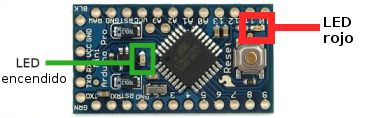
\includegraphics{led.png}
\end{center}

El LED está controlado por la señal de salida PORTB5 del microcontrolador
atmega328p, según los esquemáticos de la placa.
El manual del microcontrolador informa que esa señal es controlada por
un pin GPIO del microcontrolador, bit 5 del PORTB. Por lo tanto,
se encesita poder alternar ese pin del microcontrolador HIGH y LOW
para obtener un programa que realice el parpadeo adecuadamente.

La estructura general del programa led\_blink.c se muestra a continuación.
Esta parte del programa es independiente del hardware. De cualquier manera,
este asume que existen funciones llamadas ledInit, ledToggle, y delay\_ms
para inicializar el pin GPIO que controla el LED, cambiar el estado del LED,
y manejar el tiempo respectivamente. Esas funciones son descriptas en las 
siguientes secciones, en las que realmente le encontraremos un
sentido de lo que se siente al programar sistemas embebidos.

\begin{verbatim}
#include "led.h"

/**********************************************************************
 *
 * Function: main
 *
 * Description: Blink the green LED once a second.
 *
 * Notes:
 *
 * Returns: This routine contains an infinite loop.
 *
 **********************************************************************/
int main(void)
{
    /* Configure the green LED control pin. */
    ledInit( );

    while (1)
    {
        /* Change the state of the green LED. */
        ledToggle( );

        /* Pause for 500 milliseconds. */
        delay_ms(500);
    }

    return 0;
}
\end{verbatim}

\section *{La función ledInit}

Antes de comenzar a utilizar un periférico particular se debe entender el 
hardware utilizado para controlar ese periférico específico.

\fcolorbox{black}{grey}{
\parbox[t]{1.0\linewidth}{ \vspace*{0.4cm}
NOTA: Toda la documentación del microcontrolador ATMEL AVR atmega328p, y 
de la placa arduino pro mini se encuentra disponible. Incluye las hojas de datos,
manuales de programación, esquemáticos, etc.
\vspace*{0.4cm} } }

Como el LED que se necesita parpadear está conectado a uno de los pines
GPIO bidireccionales del microcontrolador, nos enfocamos en estos.
Frecuentemente, como es el caso con el microcontrolador atmega328p, los
pines de E/S de un procesador embebido tienen varias funciones.
Esto permite que el mismo pin sea utilizado como E/S controlable por el usuario
o para soportar funcionalidad particular dentro del procesador.
Los registros de configuración se utilizan para establecer como la aplicación
utilizará cada pin especifico de un puerto.

En el atmega328p algunos pines de un puerto pueden ser configurado para
uso por un periférico interno (llamado una funcion alternativa del pin)
o por el usuario (llamado un pin de propósito general). Por cada GPIO pin
existen varios registros de 8 bits. Estos registros
permiten configurar y controlar cada pin GPIO.
La descripción de los registros para el puerto GPIO que contiene el pin
para el LED rojo se muestra en la Tabla 3-1. Estos registros son parte
del atmega328p



\begin{center}
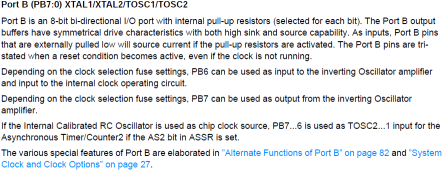
\includegraphics{descripcion-registro.png}
\end{center}



El manual del atmega328 establece que la configuración del pin GPIO para el
LED es controlado por el bit 5 del registro DDRB (Data Direction Register).
Los registros DDRX determinan si los pines se utilizarán como ENTRADA
o como SALIDA.
La Figura 3-2 muestra la ubicación del bit 5 en el registro DDRB. Este
bit configura la dirección del pin GPIO que controla el LED rojo.

\begin{center}
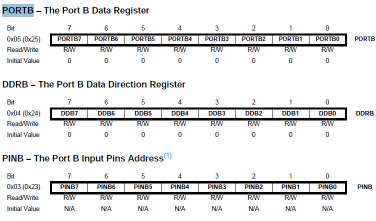
\includegraphics{portb-ddrb.png}
\end{center}

Estos registros de configuración y control están ubicados en el espacio de memoria, como se muestra en la Figura 2-6.
Las direcciones de estos registros se presentan en la Tabla 3-1. 
Debido a que los registros están mapeados en memoria se los puede
acceder facilmente en C, de la misma manera que una ubicación de memoria
es leída o escrita.

\fcolorbox{black}{grey}{
\parbox[t]{1.0\linewidth}{ \vspace*{0.4cm}
NOTA: Note, al leer el manual del atmega328, que ciertos registros
contienen bits que están etiquetados como reservados.
Esto es algo común en muchos registros dentro de un procesador.
El manual debe indicar cómo se deben leer o escribir tales bits, por
lo que es importante que no utilice esos bits para otros propósito, 
o modifique los mismos sin leer el manual.
\vspace*{0.4cm} } }


\fcolorbox{black}{grey}{
\parbox[t]{1.0\linewidth}{ \vspace*{0.4cm}
NOTA 2: Acceso a registros en espacio de E/S
Si los registros para los pines GPIO se encuentran en el espacio de E/S
se los puede acceder unicamente a través de código en lenguaje ensamblador.
EL lenguaje ensamblador para el 80x86, por ejemplo, tiene instrucciones para
acceder al espacio de E/S, llamadas in y out. EL lenguaje C no tiene
soporte nativo para estas operaciones. Funciones específicas en C
llamadas inport y outport han sido escritas, pero son parte de los
paquetes de bibliotecas estandar específicos para procesadores 80x86.
\vspace*{0.4cm} } }

La mayoría de los registros dentro de una CPU tienen una configuración
predeterminada luego de un reset.
Esto significa que antes de que se pueda controlar la salida de cualquier
pin de E/S se debe asegurar que el pin está configurado correctamente.
Luego de un reset, los pines del puerto B del atmega328 están configurados
como [ COMPLETAR esta seccion . 

\fcolorbox{black}{grey}{
\parbox[t]{1.0\linewidth}{ \vspace*{0.4cm}
NOTA: si se diera el caso que luego de un reset los pines están configurados
como se necesitan tambien se debe verificar que no exista otro software 
que no cambió la funcionalidad de estos pines GPIO (por ejemplo un bootloader).
Por lo que es una buena práctica inicializar el hardware siempre, aun
cuando se verifique que el comportamiento predeterminado es el deseado.
\vspace*{0.4cm} } }

En nuestro caso, se necesita configurar el pin GPIO 5 del puerto B como 
salida, a través del bit 5 del puerto DDRB (Data direction register).
La máscara de bits para el pin GPIO que controla el LED rojo en la
placa arduino pro mini está definido en el programa como sigue :

\begin{verbatim}
#define LED_ROJO	(0x20)		/* 0b00100000 */
\end{verbatim}

Una técnica fundamental utilizada en la rutina ledInit es la lectura-modificacion-escritura de un registro de hardware.
Primero, se lee el contenido del registro, entonces se modifica el bit que controla el LED, y finalmente, se escribe el nuevo valor de vuelta en la ubicación
del registro.
El código en ledInit realiza esta operación de lectura-modificación-escritura,
con el registro DDRB. Estas operaciones se realizan en lenguaje C utilizando
las operaciones \&= y |=. El efecto de x \& = y es el mismo que el de
x = x \& y. Se explica con un poco mas de detalle estas operaciones para manipulacion
de bits en el Capítulo 7.

La funcion ledInit configura el microcontrolador atmega328 en la placa
arduino pro mini para controlar el led rojo localizado en el centro de la placa.
En el código debajo note que se pone en cero el pin GPIO en el registro
PORTB, para asegurarnos que el voltage de salida en el pin GPIO es 
establecido a cero.


\begin{verbatim}
#define PIN22_FUNC_GENERAL (0xFFFFCFFF)

/**********************************************************************
 *
 * Function: ledInit
 *
 * Description: Initialize the GPIO pin that controls the LED.
 *
 * Notes: This function is specific to the Arcom board.
 *
 * Returns: None.
 *
 **********************************************************************/

void ledInit(void)
{
    /* Turn the GPIO pin voltage off, which will light the LED. This should
     * be done before the pins are configured. */
    GPIO_0_CLEAR_REG = LED_ROJO;

    /* Make sure the LED control pin is set to perform general
     * purpose functions. RedBoot may have changed the pin's operation. */
    GPIO_0_FUNC_HI_REG &= PIN22_FUNC_GENERAL;

    /* Set the LED control pin to operate as output. */
    GPIO_0_DIRECTION_REG |= LED_ROJO;
}
\end{verbatim}


\section *{La función ledToggle}

Esta rutina es llamada desde un bucle infinito, y es respondable de cambiar
el estado del LED. El estado del LED es controlado a través del registro
PORTB. Activando (colocando un uno) el bit 5 de este puerto cambia el voltage 
en el pin externo a 5v (HIGH), por lo que el LED rojo se enciende.
Desactivando el bit 5 de PORTB realiza la función inversa, y el voltage cambia
a 0V (LOW) y el LED se apaga.
Si se desea conocer por software si el LED está encendido o apagado simplemente
se puede leer el bit 5 de PORTB.

Como este registro (PORTB) es de lectura escritura el estado de este bit
5 puede ser cambiado con una única instrucción en C.

\begin{verbatim}
/**********************************************************************
 *
 * Function: ledToggle
 *
 * Description: Toggle the state of one LED.
 *
 * Notes: This function is specific to the Arcom board.
 *
 * Returns: None.
 *
 **********************************************************************/
void ledToggle(void)
{
    /* Check the current state of the LED control pin. Then change the
     * state accordingly. */
    if (GPIO_0_LEVEL_REG & LED_ROJO)
        GPIO_0_CLEAR_REG = LED_ROJO;
    else
        GPIO_0_SET_REG = LED_ROJO;
}
\end{verbatim}

\section *{La funcion delay\_ms}

Tambien necesitamos implementar una espera de 500ms entre el encendido y apagado
del LED. Esta acción se realiza por medio de una espera dentro de la rutina
delay\_ms.
Esta rutina acepta como entrada la longitud de la espera requerida, en milisegundos, como parámetro. Dentro se multiplica ese valor por la constante
CYCLES\_PER\_MS para obtener el número total de iteraciones que el bucle
while debe realizar, para lograr la espera en tiempo requerida.


\begin{verbatim}

/* Number of decrement-and-test cycles. */
#define CYCLES_PER_MS (9000)

/**********************************************************************
 *
 * Function: delay_ms
 *
 * Description: Busy-wait for the requested number of milliseconds.
 *
 * Notes: The number of decrement-and-test cycles per millisecond
 * was determined through trial and error. This value is
 * dependent upon the processor type, speed, compiler, and
 * the level of optimization.  
 *
 * Returns: None.
 *
 **********************************************************************/
void delay_ms(int milliseconds)
{
    long volatile cycles = (milliseconds * CYCLES_PER_MS);

    while (cycles != 0)
        cycles--;
}
\end{verbatim}

La constante especifica del hardware CYCLES\_PER\_MS representa el numero
de veces que el procesador debe iterar a través del bucle while en un milisegundo.
Para determinar este valor puede utilizar prueba y error.
En secciones futuras se explica como utilizar un contador de hardware para
alcanzar una mejor precisión de tiempo. 

Las cuatro funciones main, ledInit, ledToggle y delay\_ms realizan la tarea completa del programa que parpadea el LED. Todavia se necesita entender como construir y ejecutar este programa. En los próximos dos capítulos se explican estos temas.
Pero primero, realizamos algunos comentarios con respecto a los bucles infinitos y su rol en sistemas embebidos.

\section *{EL rol del bucle infinito}

Una de las diferencias fundamentales entre programas desarrollados para sistemas
embebidos y los desarrollados para otras plataformas de computación es que los programas
embebdos casi siempre tienen un bucle infinito.
Tipicamente, este bucle rodea una parte significativa de la funcionalidad
del programa, como sucede con el programa Blinking LED. El bucle infinito
es necesario porque el software embebido nunca finaliza.
La intención es que el programa se ejecute hasta que el mundo termine
o la plataforma es reiniciada, cualquiera que suceda primero.

Además, la mayoría de los sistemas embebidos ejecutan unicamente una sola
pieza de software. Aunque el hardware sea importante, el sistema
no es un reloj digital o un celular o un horno microondas sin el software.
Y si el software para la ejecución, el hardware se convierte en inútil.
Por lo tanto, las partes funcionales de un programa embebido están siempre
encerradas por un bucle infinito que se asegura de que el programa
se ejecutará por siempre.

Si no se coloca el bucle infinito en el programa Blinking LED el LED hubiese
parpadeado una única vez.

\section*{Referencias}

Michael Barr. Programming Embedded Systems in C and C++ 1st Edition. ISBN-13: 978-1565923546
ISBN-10: 1565923545. O'Reilly Media; 1 edition (February 9, 1999)


\include{licGASL}

\end{document}

